\documentclass[journal]{IEEEtran}

% Packages
\usepackage{graphicx}
\usepackage{cite}
\usepackage{amsmath}
\usepackage{url}
\usepackage{tikz}
\usetikzlibrary{matrix,shapes.multipart, positioning}

% Drafting Utility Package
\usepackage{comment}

% Title
\title{A Comparative Study of Techniques for Addressing Class Imbalance in Machine Learning}

\author{Brandon Hosley, 1st Lt, \textit{AFIT}%
	\thanks{Manuscript received May 16, 2023%
		%		; revised Month DD, YYYY.
}}

%\keywords{class imbalance, data-level methods, algorithm-level methods, hybrid methods, machine learning, performance evaluation}

% Document
\begin{document}
	
	\maketitle
	
	
	% Abstract
	\begin{abstract}
		Class imbalance is a pervasive challenge in machine learning, occurring when the distribution of classes in a dataset is significantly skewed. Traditional learning algorithms often struggle to accurately classify minority classes due to the dominance of majority classes. To address this issue, various techniques have been proposed to mitigate the impact of class imbalance on model performance. This paper presents a comparative analysis of different methods for handling class imbalance, aiming to provide insights into their effectiveness and suitability across a range of domains and datasets.
	\end{abstract}
	
	% Introduction
	\section{Introduction}
	\label{sec:introduction}
	Class imbalance is a pervasive challenge in machine learning, where certain classes within a dataset are significantly underrepresented compared to others. This disparity often leads to biased models that are less accurate in predicting minority class instances, resulting in suboptimal overall performance. In various real-world applications, such as fraud detection, medical diagnosis, and rare event prediction, the minority class is often more significant than the majority class. In critical domains, such as medical diagnoses, where the cost of false negatives is extremely high, failing to correctly identify instances of the minority class can have severe implications. Consequently, it is crucial to develop effective strategies that mitigate the impact of class imbalance on model performance.
	
	In recent years, researchers have proposed numerous techniques to address class imbalance and improve model performance. These methods can be broadly categorized into three main approaches: data-level methods, algorithm-level methods, and hybrid methods. Data-level methods focus on modifying the dataset itself by oversampling the minority class, undersampling the majority class, or generating synthetic samples. Algorithm-level methods aim to adapt existing machine learning algorithms or design new ones that are more robust to class imbalance. Hybrid methods combine data-level and algorithm-level techniques to leverage the advantages of both.
	
	Given the abundance of class imbalance handling methods, it becomes crucial to conduct a comparative analysis to understand their relative strengths and weaknesses. 
	% We evaluate the effectiveness of each method using a diverse set of real-world and synthetic datasets, encompassing various levels of class imbalance and problem complexities. 
	% Our assessment includes a thorough analysis of performance metrics, such as accuracy, precision, recall, F1-score, and area under the receiver operating characteristic curve (AUC-ROC), to provide a holistic understanding of the impact of each technique on model performance.
	By empirically evaluating these techniques on diverse datasets and considering different evaluation metrics, we can gain insights into their effectiveness, applicability, and trade-offs. This paper aims to bridge this gap by providing a comprehensive evaluation of 
	%state-of-the-art class imbalance handling methods.
	well-known class imbalance handling methods.
	
	By comparing and contrasting these methods, we aim to provide practitioners and researchers with valuable insights into the relative strengths and weaknesses of each technique. Moreover, our study intends to offer guidelines for selecting the most appropriate approach based on the specific characteristics of a given problem. Ultimately, we hope this work contributes to the development of more accurate and reliable selection of techniques to address disparate machine learning models in the face of class imbalance challenges.
	
	\begin{comment}
		The contributions of this study include:
		\begin{itemize}
			\item An in-depth review of existing class imbalance handling techniques, categorizing them into data-level, algorithm-level, and hybrid methods.
			\item A comparative analysis of these methods using benchmark datasets from various domains.
			\item Evaluation of the methods based on performance metrics such as accuracy, precision, recall, F1-score, and area under the receiver operating characteristic curve (AUC-ROC).
			\item Insights into the strengths, limitations, and applicability of different class imbalance handling techniques.
			\item Recommendations for selecting the most suitable method(s) based on the characteristics of the dataset and the requirements of the application domain.
		\end{itemize}
	\end{comment}
	
	The remainder of this paper is organized as follows. Section 2 provides an overview of related work on class imbalance handling methods. Section 3 describes the dataset used for experimentation and the evaluation metrics employed. Section 4 presents a description of the methodology used to perform analysis of the different class imbalance handling methods. Section 5 discusses the experimental results, comparing the performance of the methods. Finally, Section 6 concludes the paper with a summary of the findings, limitations of the study, and potential directions for future research.
	
	% Literature Review
	\section{Related Work}
	\label{sec:related_work}
	
	
	
	\subsubsection{Undersampling}
	
	
	
	
The earliest and most straightforward approaches to deal with class imbalance involve resampling the dataset. Undersampling techniques, such as random undersampling (RUS) and Tomek Links, reduce the instances of the majority class to balance the class distribution Liu et al. \cite{liu2009}. 

\subsection{Oversampling}

On the other hand, oversampling techniques such as random oversampling (ROS) and Synthetic Minority Over-sampling Technique (SMOTE) Chawla et al. \cite{chawla2002} increase the instances of the minority class. However, these methods can lead to overfitting (oversampling) or loss of potentially important data (undersampling).

\subsection{Cost-Sensitive Learning}

Cost-sensitive learning (CSL) is another strategy that assigns higher misclassification costs to the minority class Elkan et al. \cite{elkan2001}. This method avoids the overfitting problem of oversampling and the information loss of undersampling. However, the performance of CSL is dependent on the cost matrix, which is often hard to determine.

\subsection{Ensemble Methods} 
Ensemble methods, like Boosting and Bagging, have been extensively used to address class imbalance. AdaBoost Freund et al. \cite{freund1997} is a popular boosting algorithm, while Balanced Random Forests Chen et al. \cite{chen2004} is a well-known bagging technique. Both methods construct multiple classifiers and combine them to make the final decision. These techniques have been proven effective, but they can be computationally expensive.

\subsection{Learning from Imbalanced Data Streams} 
Imbalanced data streams are a more challenging scenario where the data distribution may change over time. Wang et al. \cite{wang2018} proposed a method that dynamically adjusts the class distribution by a resampling strategy. Gao et al. \cite{gao2015} presented a method that incrementally learns from the data stream by adjusting the decision boundaries.

\subsection{Deep Learning Approaches}
With the recent advancement in deep learning, several methods have been proposed to handle class imbalance. Cui et al. \cite{cui2019} introduced a loss function, called Class-Balanced Loss, based on effective number of samples. This technique achieves a balance between classes by adjusting the weights in the loss function. Similarly, Khan et al. \cite{khan2017} proposed Cost-Sensitive Deep Learning, which incorporates the cost matrix into the loss function of the deep learning model.

These methods illustrate the wide range of techniques that have been proposed to tackle class imbalance. In this paper, we compare these methods on a suite of benchmarks to provide insights into their relative strengths and weaknesses.
	
	
	% Dataset
	\section{Dataset}
	\label{sec:dataset}
	
	\subsection{CDC Diabetes Dataset}
	\cite{cdc2022}
	Diabetes is a prevalent chronic disease in the U.S. that affects millions of individuals, resulting in a significant economic impact. Complications include heart disease, vision loss, limb amputation, and kidney disease. Despite the absence of a cure, weight loss, healthy eating, physical activity, and medical treatments can manage the disease. Early diagnosis and predictive models are crucial for effective treatment and lifestyle modifications.
	
	The CDC conducts an annual health-focused telephone survey known as the Behavioral Risk Factor Surveillance System (BRFSS). Initiated in 1984, the survey garners responses from over 400,000 Americans each year, gathering data on health-related risk behaviors, chronic health conditions, and utilization of preventive services. For the project at hand, we used a dataset derived from the 2015 version survey, available on Kaggle as a csv file. The raw dataset comprised responses from 441,455 individuals and included 21 features derived from 330 questions, which are a combination of direct questions posed to participants and variables calculated based on their responses.

	The derived dataset was cleaned and balanced leaving 70,692 samples with 17 features and one response variable. 
	
	
	% Methodology
	\section{Methodology}
	\label{sec:methodology}




In our final pre-processing for the diabetes dataset

dropped features with extremely low variance,
in this case heavy alcohol consumption and stroke.
the positive cases were extremely small

'Sex','Smoker','Fruits','Veggies'
low correlation with the response var

Leaving 6 features
which were scaled.

Then used.



\begin{figure}
	\centering
	\begin{tikzpicture}
		\node[inner sep=0pt] (image) at (0,0)
		{\includegraphics[width=0.5\textwidth]{4Lrff}};
		\node[red!50!black, font=\Huge\bfseries, rotate=45] at (image.center) {Temporary Example};
	\end{tikzpicture}
	\caption{TikZ diagram is under construction.}
	\label{fig:4lrff}
\end{figure}






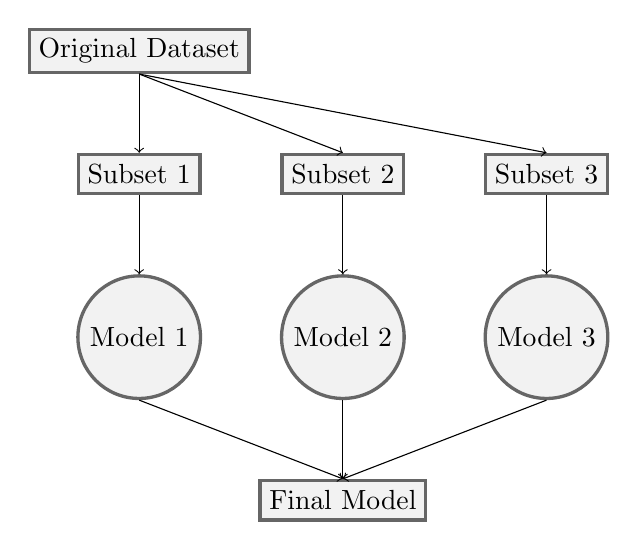
\begin{tikzpicture}[
	roundnode/.style={circle, draw=black!60, fill=black!5, very thick, minimum size=7mm},
	squanode/.style={rectangle, draw=black!60, fill=black!5, very thick, minimum size=5mm},
	]
	
	%Nodes
	\node[squanode] (Maintable)     {Original Dataset};
	\node[squanode] (Subset1) [below=of Maintable] {Subset 1};
	\node[squanode] (Subset2) [right=of Subset1] {Subset 2};
	\node[squanode] (Subset3) [right=of Subset2] {Subset 3};
	\node[roundnode] (Model1) [below=of Subset1] {Model 1};
	\node[roundnode] (Model2) [below=of Subset2] {Model 2};
	\node[roundnode] (Model3) [below=of Subset3] {Model 3};
	\node[squanode] (FinalModel) [below=of Model2] {Final Model};
	
	%Lines
	\draw[->] (Maintable.south) -- (Subset1.north);
	\draw[->] (Maintable.south) -- (Subset2.north);
	\draw[->] (Maintable.south) -- (Subset3.north);
	\draw[->] (Subset1.south) -- (Model1.north);
	\draw[->] (Subset2.south) -- (Model2.north);
	\draw[->] (Subset3.south) -- (Model3.north);
	\draw[->] (Model1.south) -- (FinalModel.north);
	\draw[->] (Model2.south) -- (FinalModel.north);
	\draw[->] (Model3.south) -- (FinalModel.north);
	
\end{tikzpicture}

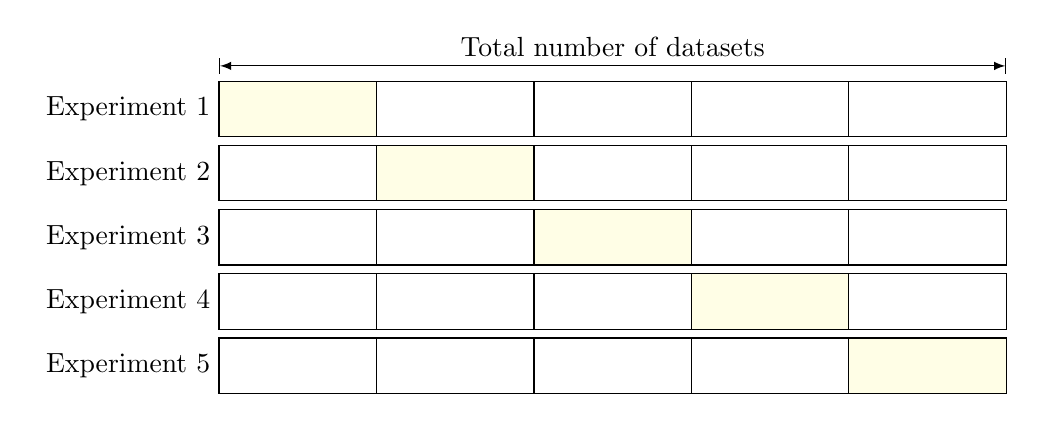
\begin{tikzpicture}
\matrix (M) [matrix of nodes,
nodes={minimum height = 7mm, minimum width = 2cm, outer sep=0, anchor=center, draw},
column 1/.style={nodes={draw=none}, minimum width = 4cm},
row sep=1mm, column sep=-\pgflinewidth, nodes in empty cells,
e/.style={fill=yellow!10}
]
{
	Experiment 1 & |[e]| & & & & \\
	Experiment 2 & & |[e]| & & & \\
	Experiment 3 & & & |[e]| & & \\
	Experiment 4 & & & & |[e]| & \\
	Experiment 5 & & & & & |[e]| \\
};
\draw (M-1-2.north west) ++(0,2mm) coordinate (LT) edge[|<->|, >= latex] node[above]{Total number of datasets} (LT-|M-1-6.north east);
\end{tikzpicture}



	% Results and Discussion
	\section{Results and Discussion}
	\label{sec:results_discussion}
	This section presents the results obtained from the project and discusses them in detail. It may include tables, figures, graphs, or charts to present the findings. The results are analyzed, interpreted, and compared with existing work or expected outcomes. The implications, limitations, and potential future directions are also discussed.
	
	% Conclusion
	\section{Conclusion}
	\label{sec:conclusion}
	This section summarizes the key findings, contributions, and implications of the project. It restates the project objectives, highlights the accomplishments, and discusses the significance of the work. It may also suggest areas for further research or improvements.
	
	\subsection{Future Work}
	More than a binary classification
	Additional techniques
	
	% References
	\section*{References}
	\label{sec:references}
	\bibliographystyle{IEEEtran}
	%\bibliography{references}
	
\end{document}
